\section{Balance Workload}
\label{sec:balanceworkload}
Whenever a staff member is removed from a department or has marked a problem as solved, 
it becomes necessary to balance the workload of each staff member in the department, since we do not want the staff members to be overloaded with problems. 

To balance the workload, each staff members workload must be calculated. 
The workload of a staff member is defined by the amount of time estimated that each problem on his workload takes to be solved. 
The workload is calculated by the \me{GetWorkload} method.

The time a problem takes to be solved is estimated by the average time consumption of the tags connected to the problem. 
This is calculated by the \me{CalculateTimeConsumption} method.

The \me{BalanceWorkload} method works by finding the staff member in the department with the minimum workload and the staff member with the maximum workload. Then it moves the problem with the lowest estimated time consumption from the maximum staff member to the minimum. 
It keeps reassigning problems until the minimum staff member has a higher or equal workload than the maximum staff member. If the minimum staff member has a higher workload, then the algorithm checks if the balance can be balanced even further by calculating if the last moved problem should be moved back or not, and moves it accordingly. See lines 25 to 42 in code snippet \ref{lst:balanceWorkload}.

%The original idea was that this would ensure that bad last reassignments would be omitted by switching them backwards. However, later we discovered that this approach is not sufficient to prevent bad last reassignments. An example is illustrated in figure \ref{fig:balanceWorkload_strangecase}. The dark grey colored box is representing a high priority problem which in the first scenario, the workload is most balanced if it is moved back after the final iteration of the loop, whereas the workload is most balanced if it is not moved back in on the scenario to the right, marked ``Move back Bad idea''. Although that this seems like a trivial bug to fix afterwards, we chose not to fix it, as it would make.

All this is iterated once per staff member minus one in the department. 
E.g. if there are two staff members it is ran once, if there is three it yields two etc. 
The pseudo code is displayed in code snippet \ref{lst:balanceWorkload}.

The primary concern of the algorithm is to distribute the problems so each staff member has as balanced workload as possible.

 
%This balance is based on the time of all the individual staff members problems are approximated to take.
%This balance is based on the time approximated that all problems on his workload consumes. 
%							den tid alle de individuelle staff medlemmers problemer er approximeret til at tage, tilsammen.
%Balancen er baseret p\aa{} den tid alle staff problemer er approximeret til at tage tilsammen. 


%We also wanted the algorithm to take the individual priority of the problems into account. 
%This algorithm makes sure that the high priority problems will be distributed. 
%If the priority was unrelevant the algorithm would take the problem with lowest time consume, since this would give the most balanced workload. 
An example of the algorithm is shown on figure \ref{fig:balanceWorkloadDiagram}. 

%There is one weakness though and that is if a staff has a highly time consuming problem with low priority. Then he will be left with only that problem. Assuming it is as time consuming as all the other problems. 



\begin{figure}
	\centering
		%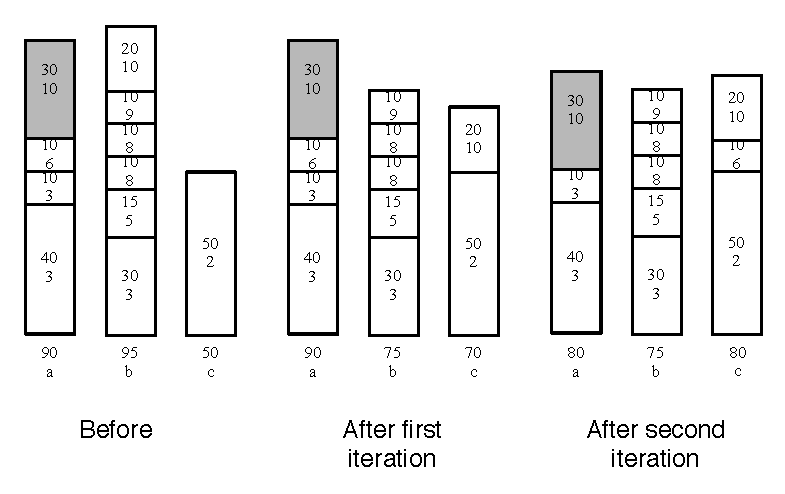
\includegraphics[scale=0.8]{input/implementation/key_points/balanceWorkloadDiagram.pdf}
	\morscaption{A diagram of the balance workload method. Each collumn represents a staff members workload. Each box is a problem. The height represents the estimated time consumption. The problem colored dark grey is not reassignable.  There are tree staff members a, b, and c. The problems that will be moved is colored light grey.}
	\label{fig:balanceWorkloadDiagram}
\end{figure}



\begin{lstlisting}[style=sourceCode, caption=\myCaption{A code snippet of the balance workload method. The presented code is within a for loop running for each staff member minus one. ``min'' and ``max'' are the person objects of which the algorithm are currently moving problems between. \vari{maxWorklistist} a sorted worklist. It is sorted in non-deacreasing order according to the estimated time consumption. }, label=lst:balanceWorkload]
bool couldStillMove = true;
do
{
    // Finde the reassignable problem with the highest priority which has not been moved yet. 
    var problemToBeMoved = maxWorklist.FirstOrDefault(y =>
	    y.Reassignable == true &&
	    y.HasBeen == false &&
	    y.SolvedAtTime == null);
                  
    // If none can be moved leave the while loop
    if (problemToBeMoved == null)
    {
        couldStillMove = false;
    }
    else
    {
        // Mark as has been moved
        problemToBeMoved.HasBeen = true;

        // Reassign the highest priority problem to staff member called min.
        problemToBeMoved.AssignedTo = min;

        if (min.Workload >= max.Workload)
        {
            // Initialize variables for checking whether or not to move the last problem back
            double beforeMoveBack = 0.0;
            double afterMoveBack = 0.0;

            // Calculate difference before moving
            beforeMoveBack = Math.Abs(max.Workload - min.Workload);

            // Move it back
            problemToBeMoved.AssignedTo = max;

            // Calculate difference after moving
            afterMoveBack = Math.Abs(max.Workload - min.Workload);

            // Compare
            if (beforeMoveBack < afterMoveBack)
            {
                problemToBeMoved.AssignedTo = min;
            }
            couldStillMove = false;
        }
        else if (min.Workload == max.Workload)
        {
            // Don't move back if they are equal
            couldStillMove = false;
        }
    }
} while (couldStillMove);



\end{lstlisting}


